\chapter{Testrig}
\section{Introduction}
When designing a complex system such as a hybrid vehicle, continuously being
able to test the system is important to validate that the requirements are met
and to verify the models. To be able to do a full system test, the car has to be
physically run on a track. This can be cumbersome, or in the case of the London
track, impossible at times. Therefore, a test rig is designed and built. The
design process uses the V-model approach with a set of live requirements and
continuous unit and integration testing. The overall goal is to not only be able
to do a faithful simulation of the EcoCar track in London, but to be able to
supply any track (with certain limitations on power and speed demands) to the
test rig and simulations on the car.

\section{Requirements}
The requirements on the test rig are designed to capture the essential demands
on the system. Firstly, the high level User requirements are set. These are set
to capture the problem and to describe the goal of designing the system
~\cite{ibm_req}. The User requirements are then developed into the System
requirements that describe the limitations and demands on the system and its
subsystems.

\section{Hardware}
The testrig is composed of two rollers mounted on a metal frame together with a DC motor as well as an incremental quadratic encoder to keep track of the speed of the motor. The motor is connected to the rollers by sprockets and chain with a gearing ratio of two. To control the DC motor an Arduino Mega microcontroller calculates what current should be applied to the motor, this reference signal is used by a ESCON driver to control the current in a local feedback loop.

To create a braking torque on the test rig it is needed to generate a current from the DC motor that has to be handled somehow, since the motor will work as a generator while braking. This was done by the manufacturing of a system that stores the energy created, and if more energy is created than the system can handle, energy is sent to six parallel power resistors that will burn off the excess energy. 

The current from the DC motor is sent to a supercapacitor that is connected directly to the motor driver, where the created energy is stored. Since the driver needs to have a relatively stable input voltage, we want the threshold of the voltage on the supercapacitor to be stable. Therefore it was decided to start burning energy if the voltage exceeds 47 volt. The voltage cannot drop too much either, therefore a power supply unit was added as a backup if we need to simulate a steep downhill where the motor will act as a motor instead of a generator, and therefore draw current instead of generating. 

The voltage level on the supercapacitor is monitored by the microcontroller that controls what track to input to the driver. If the voltage exceeds 47 volt the microcontroller will close a relay between the power resistors and ground, and it will remain closed until the supercap has discharged to 45 volt where the microcontroller will open the relay and make the supercapacitor able to recharge again. A basic schematic of the setup can be seen in Figure \ref{fig:testrig_schematic}.

\begin{figure}[H]
    \label{fig:testrig_schematic}
    \centering
    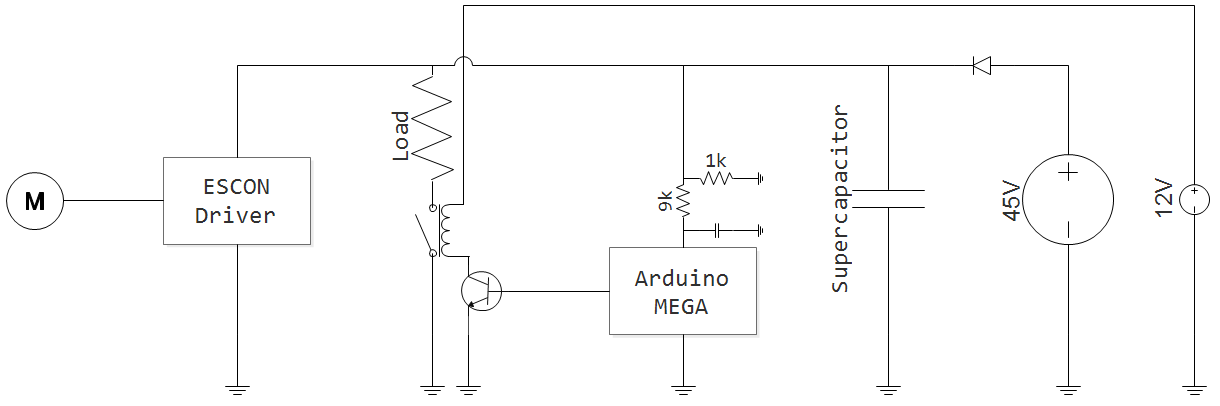
\includegraphics[width=\textwidth]{./img/testrig_schematic.png}
    \caption{Schematic of testrig wiring.}
\end{figure}

\section{Car dynamics} \label{sec:cardynamics}
The calculations in this section are in many ways the same as the calculations
given in the previous teams report in Appendix~\ref{app:elba2015}. Though some
of the equations are repetition of what was done last year, they are
done here again with some improvements and more references to make the
derivations of the equations clearer.

When simulating a track, one needs to know the force exerted by the environment
on the car. A graphical representation of the forces that act on the car is
given in Figure~\ref{fig:testrig_elbadynamics}.
\begin{figure}[H]
    \label{fig:testrig_elbadynamics}
    \centering
    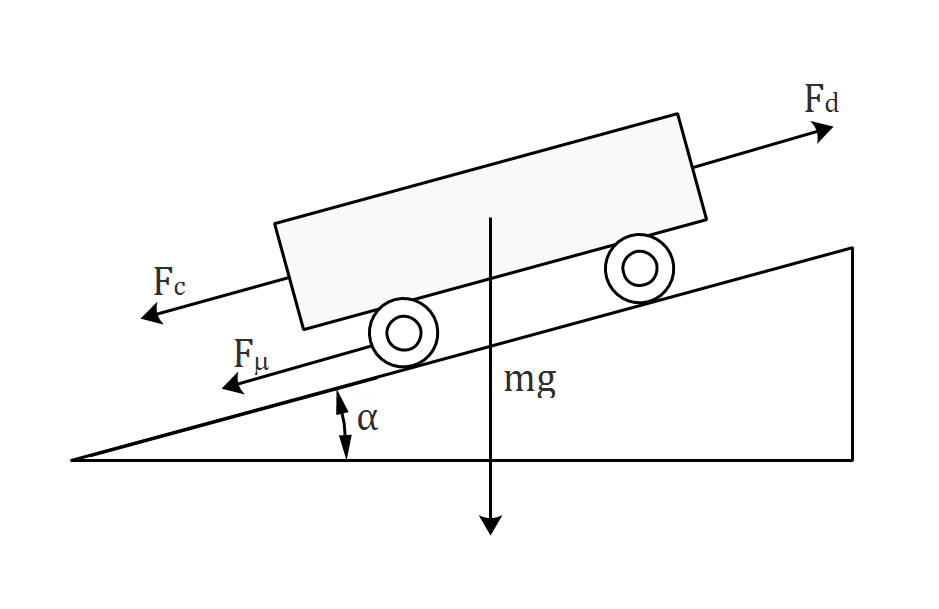
\includegraphics[width=0.5\textwidth]{./img/testrig_elbaforces.png}
    \caption{Dynamic model of Elba.}
\end{figure}
The motion equations on the system are 
\begin{equation} \label{eq:testrig_cardynamics}
    m\ddot{x} = F_d - mg\sin{\alpha} - F_c - F_{\mu},
\end{equation}
where $F_d$ is the effective driving force of the car, $m$ is the mass of the
car and $alpha$ is the slope from the horizontal plane. The resistance terms
$F_c$ and $F_{\mu}$ are air and road resistance, respectively. The air drag $D$
around an object can be calculated as \cite{nakayama2002}
\begin{equation} \label{eq:testrig_airdrag}
    D = C_D A \frac{\rho v^2} {2}
\end{equation}
with object velocity $v$, surface area vertical to the movement direction $A$
and air density $\rho$. Most terms in Equation~(\ref{eq:testrig_cardynamics})
are constant throughout a driving instance. Rewriting to
\begin{equation} \label{eq:testrig_csimple}
    C_{tot} = \frac{C_D A \rho} {2}
\end{equation}
yields a simplified equation that only depends on the velocity,
\begin{equation} \label{eq:drag}
    F_D = C_{tot}v^2.
\end{equation}
The total drag coefficient $C_{tot}$ will depend on the vertical area, the density of
air and the drag coefficient $C_D$. The air density is considered to be constant
and is known. The area of Elba can be estimated using simple methods. Finally,
the air drag coefficient $C_D$ is unique to each and every object and is
determined experimentally. For this project, the estimations given for a
passenger car is used. Detailed calculations and values are given in
Appendix~\ref{app:rigdata}. 

% This section is under construction. Need some reference/experiment on how to 
% model rolling friction.
The rolling friction of a car is modeled as a stepfunction, being non-zero at
all velocities that are not zero.

With the air drag, rolling friction and gravity terms known, only two terms of
Equation (\ref{eq:testrig_cardynamics}) are unknown. To fully model the cars
dynamics, the inerta term needs to be modeled. Since the weight of the vehicle
is known, $\ddot{x}$ needs to be derived for an accurate system model.
Knowing the radius of the rollers and the cars wheels, the linear acceleration
can be calculated by measuring the rotational acceleration on the roller. This
is done by an incremental encoder on the roller shaft. Rotational speed is
calculated in the microcontroller and rotational acceleration is derivated from
rotational speed. Using the roller radius, $r_{r}$, the linear acceleration
is calculated.

Rewriting Equation (\ref{eq:testrig_cardynamics}), (\ref{eq:drag}) and the friction force gives the
desired linear testrig simulation force on the right hand side,
\begin{equation} \label{eq:simulationforce}
    F_{tr} = m\ddot{x} + mg\sin{\alpha} + C_{tot}\dot{x}^2 + F_{\mu}.
\end{equation}

Using the height profile of the London track and the plant model of Elba, $F_{tr}$ during an entire lap could be simulated, as shown in Figure (\ref{fig:testrig_negative_forces}).

\begin{figure}[H]
    \label{fig:testrig_negative_forces}
    \centering
    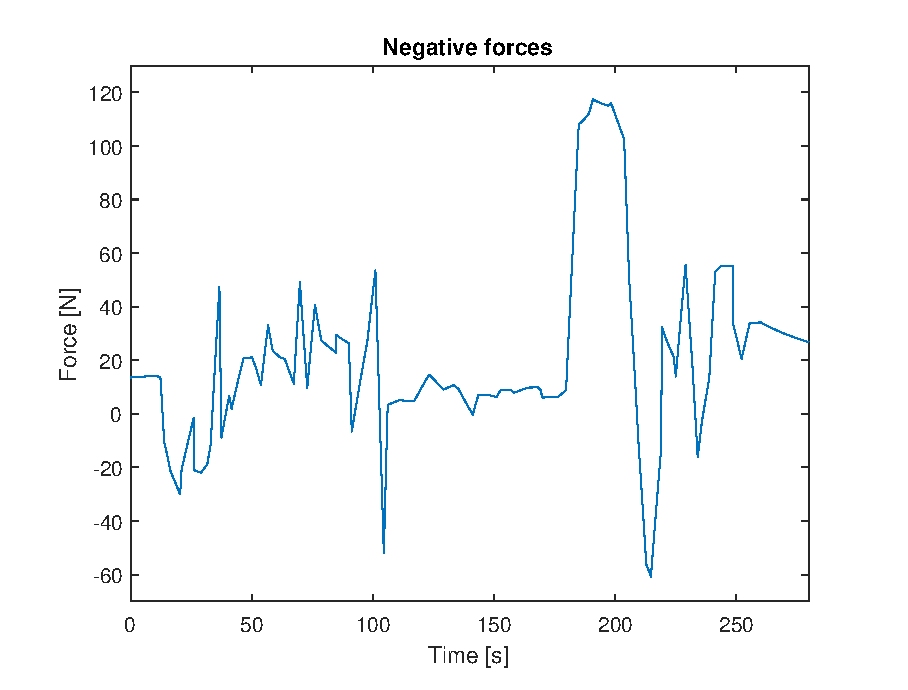
\includegraphics[width=\textwidth]{./img/testrig_negative_forces.eps}
    \caption{Negative forces acting upon Elba in one lap.}
\end{figure}

\section{Testrig dynamics}
In order to let the testrig output the correct linear force to the car, the
controller for the testrig need to know the dynamics of the testrig itself. This
is to compensate for internal frictions and inertias. The driveline of the
testrig has two separate steps, the motor and the roller, connected by a chain
gear with gear ratio $n_{chain}$. A prinicple schematic of the testrig from
motor to roller is displayed in Figure~\ref{fig:testrig_testrigdynamics}.
\begin{figure}[H]
    \label{fig:testrig_testrigdynamics}
    \centering
    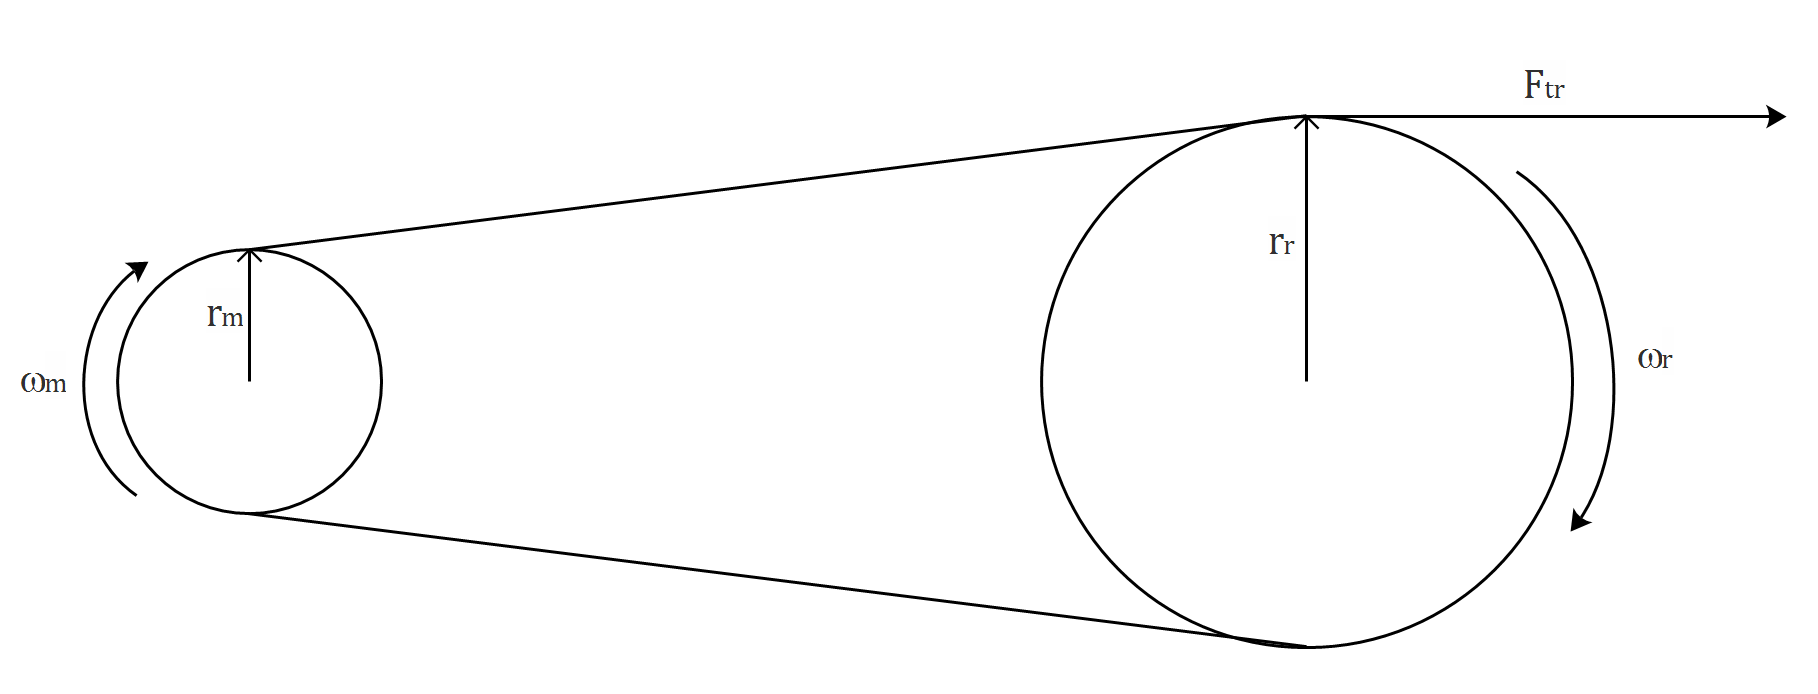
\includegraphics[width=0.9\textwidth]{./img/testrig_rollerschematic.png}
    \caption{Principle schematic of the testrig from motor to roller.}
\end{figure}
The dynamic equations for the rollers are
\begin{equation} \label{eq:testrig_rollerdynamics}
    J_r \dot{\omega}_r = F_{tr}r_r - d_r \omega_r - \mu_r,
\end{equation}
%Inte 100% säker på att Ftr blir rätt här /Emil

where $J_r$ is the inertia of the rollers and $\omega_r$ is the rotational velocity
of the roller. The frictional terms are the viscous friction $d_r$ and the
constant friction $\mu_r$ which is modelled by the Karnop model (??).

Connecting the rollers and the motor is a chain gear. It is modelled as a
generic gear box. The gearbox model has no internal friction. There is always friction in a
chain gear but it is expected that this friction will be incorporated in the
total system model and the friction free representation is deemed adequate.
Using Equation (\ref{eq:testrig_rollerdynamics}) and (motor model) along with
the gearbox model, the total testrig dynamic model becomes

\begin{equation} \label{eq:testrig_totaldynamics} 
    T_m = \frac{F_{tr} r_r + J_{tot} \dot{\omega}_m + d_{tot} \omega_m + \mu_{tot}}{n},
\end{equation}

%TODO: Kanske fel i ekvationen, möjligt korrekt:
%\begin{equation} \label{eq:testrig_totaldynamics2} 
%    T_m = \frac{F_{tr} r_w + J_{tot} \dot{\omega}_m + d_{tot} \omega_m + \mu_{tot}}{n_1 n_2},
%\end{equation}

with motor torque $T_m$, simulation force $F_{tr}$ and motor rotational velocity
$\omega_m$. The inertia term is the combined inertia of the motor and
roller,
\begin{equation} \label{eq:totalinertia}
    J_{tot} = J_m + J_r \frac{1} {n^2}.
\end{equation}
The friction terms are combined terms as well, namely
\begin{equation} \label{eq:testrig_totalvfric}
    d_{tot} = d_m + d_r \frac {1} {n}
\end{equation}
and
\begin{equation} \label{eq:testrig_totalfric}
    \mu_{tot} = \mu_m + \mu_r.
\end{equation}

The power $P_m$ required for the motor on the testrig was calculated as
\begin{equation} \label{eq:testrig_motorpower}
	P_m = T_m \omega_m
\end{equation}

Using the London track and the plant model of Elba, $P_m$ during one lap could be simulated, as shown in (\ref{fig:testrig_power_required}).

\begin{figure}[H]
    \label{fig:testrig_power_required}
    \centering
    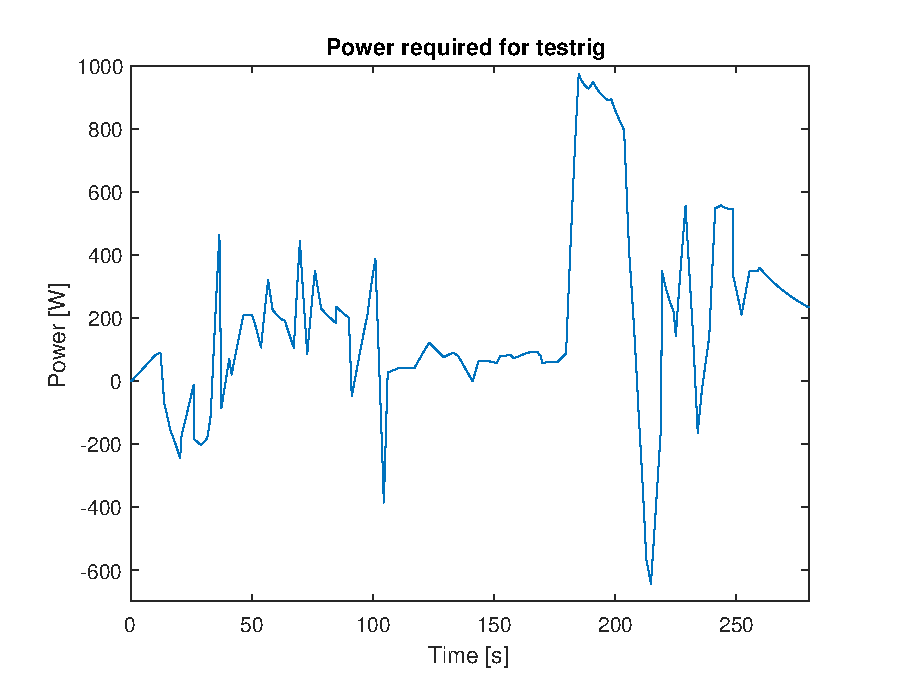
\includegraphics[width=\textwidth]{./img/testrig_power_required.eps}
    \caption{Power required for the motor on the testrig.}
\end{figure}

Figure (\ref{fig:testrig_power_required}) shows that the maximum required power from the testrig motor is $1000$ W.

\section{Identification}
Having obtained the dynamic equations of the system in Equation
(\ref{eq:testrig_totaldynamics}), a system identification is done to determine
the parameters of the system. The parameters are then used in the open loop
current/torque controller. The controller is run in open loop for the
torque, i.e. there is no direct torque feedback. To get the desired torque
output, the current is controlled via a closed loop feedback controller and
torque is calculated from the actual current. With a knowledge about motor
parameters and the dynamics of the system, the actual torque can be estimated. 

\subsection{Hardware setup}
The testing is processed in Matlab and Simulink. Input data is gathered from the
real system and is then fed into the model afterwards for model comparison. This
has the advantage of doing a physical test once, recording the data and the be
able to test it on the model without setting up the test system again. Output
data from the testrig, rotational velocity of the motor, is also collected and
used as a reference for the model.

To measure motor voltage, a computer oscilloscope was used (Digilent Analog
Discovery 2). The oscilloscope has an open C API, allowing its interface to be
customized. An S-Function block was made that allowed the oscilloscopes
measurements to be directly recorded in Simulink. To make sure that the model
ran in real-time in Simulinks normal mode, a Real-time constraint block was
added to the simulink model. The probes of the oscilloscope were attached to
the positive and negative pole of the motor. All data was recorded into a
Simulink Datastruct that could then be used as input for the model. 

For recording the output data, rotational velocity, an incremental quadrature
encoder was used. The encoder pulse data was recorded and converted into
velocity by the test rig ECU. The Simulink model for the ECU was run on external
mode and encoder data was saved. 

Because of software limitations, the oscilloscope and the testrig ECU can not be
run in the same Simulink instance. This means that two separate models are run
simultaneously, one recording the input and one recording the output.

\subsection{Identification process}
To be able to identify the parameters of the testrig, the dynamic model from
Equation (\ref{eq:testrig_totaldynamics}) is combined with that of a DC motor. A
principle schematic of a DC motor is given in
Figure~\ref{fig:testrig_dcmotor_model}. $V_A$ is the voltage input, $R_A$ and
$L_A$ are the internal resistance and inductance respectively, $i_a$ is the
motor current and $V_C$ is the back-emf. $J$ is the inertia of the motor and
$\omega_a$ is the rotational velocity.
\begin{figure}[H]
	%TODO: Need a better picture!
    \label{fig:testrig_dcmotor_model}
    \centering
    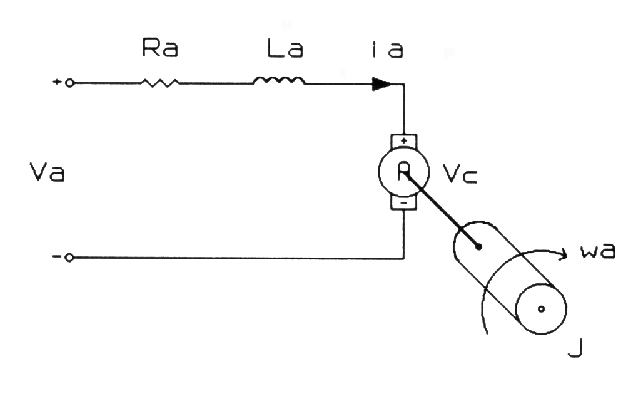
\includegraphics[width=\textwidth]{./img/testrig_dcmotor_model.png}
    \caption{DC motor schematic diagram.}
\end{figure}
Using Kirchoffs loop rule along with 
\begin{equation} \label{eq:testrig_kphi_v}
    V_C = k_{\phi} \omega
\end{equation}
and 
\begin{equation} \label{eq:testrig_kphi_i}
    T = k_{\phi} \omega
\end{equation}
gives the electric dynamics of the motor,
\begin{align} 
    V_A = R_A i_a + L_A \frac{di_a}{dt} + k_{\phi}\omega \label{eq:testrig_dcmotor_v}\\
    J \frac{d\omega} {dt} = k_{\phi} i_a - d\omega - \mu. \label{eq:testrig_dcmotor_j}
\end{align}
Performing a Lablace transform and rewriting Equation (\ref{eq:testrig_dcmotor_v}) and (\ref{eq:testrig_dcmotor_j})
one gets a second order model for the motor as a transfer function between
voltage and rotational velocity,
\begin{equation} \label{eq:testrig_motor_2ndorder}
    \omega = \frac {k_{\phi}} {(sJ + d)(R_A + sL_A) + k_{\phi}^2} U_A.
\end{equation}
In order to reduce the model complexity, $L_A$ is assumed to be small enough to
have any significant effect on the systems dynamics. With this assumtion,
Equation (\ref{eq:testrig_motor_2ndorder}) becomes a first order system,
\begin{equation} \label{eq:testrig_motor_1storder}
    \omega = \frac {k_{\phi} {sJ + d R_A + k_{\phi}^2}} U_A.
\end{equation}
Equation (\ref{eq:testrig_motor_1storder}) can be rearranged to a standard first
order transfer function form yielding
\begin{equation} \label{eq:testrig_motor_1storder_rewrite}
    \omega = C_1 \frac {1} {s C_2 + 1}
\end{equation}
where $C_1 = k(1 + \frac{1} {R d})$ and $C_2 = \frac {J} {\frac{k^2} {R} + d}$.
Using the final value theorem, setting $s = 0$, $C_1$ can be seen to be the steady
state gain of the system and $C_2$ is the time constant. 


